% Copyright (C) 2005-2015 Airbus - EDF - IMACS - Phimeca
% Permission is granted to copy, distribute and/or modify this document
% under the terms of the GNU Free Documentation License, Version 1.2
% or any later version published by the Free Software Foundation;
% with no Invariant Sections, no Front-Cover Texts, and no Back-Cover
% Texts.  A copy of the license is included in the section entitled "GNU
% Free Documentation License".
\renewcommand{\filename}{docUC_StochProc_Field.tex}
\renewcommand{\filetitle}{UC : Manipulation of a field}

% \HeaderNNIILevel
\HeaderIILevel
%\HeaderIIILevel

\label{UCField}

\index{Stochastic Process!Field}



The objective here is to create and manipulate a field. A field is the agregation of a mesh $\cM$ of a domain $\cD \in \Rset^n$ and a sample of values in $\Rset^d$ associated to each vertex of the mesh. \\

We note $(\vect{t}_0, \dots, \vect{t}_{N-1})$ the vertices of $\cM$ and $(\vect{x}_0, \dots, \vect{x}_{N-1})$ the associated values in $\Rset^d$.\\

The spatial mean of a field is  defined by:
\begin{align}\label{spatMeanField}
  \displaystyle \frac{1}{N} \sum_{i=0}^{N-1} \vect{x}_i
\end{align}

%For version after 1.3:
%\begin{align}\label{spatMeanField}
%\displaystyle \frac{1}{V} \sum_{S_i \in \cM} \left( \frac{1}{d+1}\sum_{k=0}^{d} \vect{x}_{i_k}\right) |S_i|
%\end{align}
%where $S_i$ is the simplex of index $i$ of $\cM$, $|S_i|$ its volume and $(\vect{x}_{i_0}, \dots, \vect{x}_{i_d})$ the values of the field associated to the  vertices pf $\cS_i$, and $\displaystyle V=\sum_{S_i \in \cD} |S_i|$.\\
%(\ref{spatMeanField}) is an estimation of the spatial mean of the process $X$ defined in (\ref{spatMean}).



It is possible to export the field into the VTK format thanks to the method \emph{exportToVTKFormat}, which allows to visualize it using e.g. ParaView: see Figure \ref{Field3}.\\

A field is stored in the \emph{Field} object that stores the mesh and the  values at each vertex of the mesh.\\

The spatial mean is evaluated thanks to the method \emph{getSpatialMean}. When the mesh $\cM$ is a regular time grid, the spatial mean corresponds to a temporal mean which is also evaluated with the method \emph{getTemporalMean}.\\

Note that if the mesh is of dimension 1 or 2, it is possible to draw one marginal of the field as follows, where the marginal is noted $j\in[0,d-1]$:
\begin{itemize}
\item \emph{drawMarginal(j,False)} draws the marginal $j$ of the field with no interpolation between the points. Then, in dimension 1, we get the cloud $(t_i, v_i^j)_{0 \leq i \leq N-1}$. In dimension 2, we draw a bullet on each vertex $\vect{t}_i\in \cM$  which color depends on the value of the process $v_i^j$: see Figure~\ref{Field1}.
\item \emph{drawMarginal(j)} draws the marginal $j$ of the field with linear interpolation between the points: see Figure \ref{Field2}.
\end{itemize}




A field can be obtained as a realization of a multivariate stochastic process  $X: \Omega \times \cD \rightarrow \Rset^d$   of dimension $d$ where $\cD \in \Rset^n$, when the realization is discretized on the mesh $\cM$ of $\cD$. The  values $(\vect{x}_0, \dots, \vect{x}_{N-1})$ of the field are defined by:
\begin{align}
  \forall i \in [0, N-1],\quad   \vect{x}_i= X(\omega)(\vect{t}_i)
\end{align}
%For version  1.3 only:
If each simplex of the mesh has the same volume, then the spatial mean (\ref{spatMeanField}) is an estimation of the spatial mean of the process $X$ defined in (\ref{spatMean}). \\
%%%%%%%%%%%%%
% For version after 1.4:
%The spatial mean (\ref{spatMeanField}) is an estimation of the spatial mean of the process $X$ defined in (\ref{spatMean}). \\

If the mesh $\cM$ can be interpreted as a regular time grid, then the spatial mean (\ref{spatMeanField}) is an estimation of the temporal mean of the process $X$ defined in (\ref{tempMean}). \\



\requirements{
  \begin{description}
  \item[$\bullet$] a mesh : {\itshape myMesh}
  \item[type:]  Mesh
  \end{description}

  \begin{description}
  \item[$\bullet$] some values : {\itshape myValues}
  \item[type:]  NumericalSample
  \end{description}


  \begin{description}
  \item[$\bullet$] a process: {\itshape myProcess}
  \item[type:]  Process
  \end{description}

  \begin{description}
  \item[$\bullet$] the mesh of the field:  {\itshape myMesh}
  \item[type:]  Mesh
  \end{description}

  \begin{description}
  \item[$\bullet$] the values of the field:  {\itshape myValues}
  \item[type:]  NumericalSample
  \end{description}

}
{
  \begin{description}
  \item[$\bullet$] two fields:  {\itshape myField, myField2}
  \item[type:]  Field
  \end{description}

  \begin{description}
  \item[$\bullet$] the spatial mean:  {\itshape mySpatMean}
  \item[type:]  NumericalPoint
  \end{description}

  \begin{description}
  \item[$\bullet$] a value of the field:  {\itshape myValue\_i}
  \item[type:]  NumericalPoint
  \end{description}

  \begin{description}
  \item[$\bullet$] the values of the field:  {\itshape myGeneratedValues}
  \item[type:]  NumericalSample
  \end{description}
}

\textspace\\
Python script for this UseCase :

\inputscript{script_docUC_StocProc_Field}


Consider the temporal normal process of dimension~1 which covariance model is $Exponential(a,\lambda)$ with $(a, \lambda)=(1.0, 0.2)$ and the  bidimensional mesh  which is the box $[0,2]\times [0,1]$ regularly discretized with 80 points in the first dimension and 40 points in the second one. \\
We draw  a realization of this process on the mesh using no interpolation: see  Figure \ref{Field1} and using a linear interpolation: see  the Figure \ref{Field2} .\\
The Figure \ref{Field3}  shows the field as visualized using ParaView.


\begin{figure}[H]
  \begin{minipage}{6cm}
    \begin{center}
      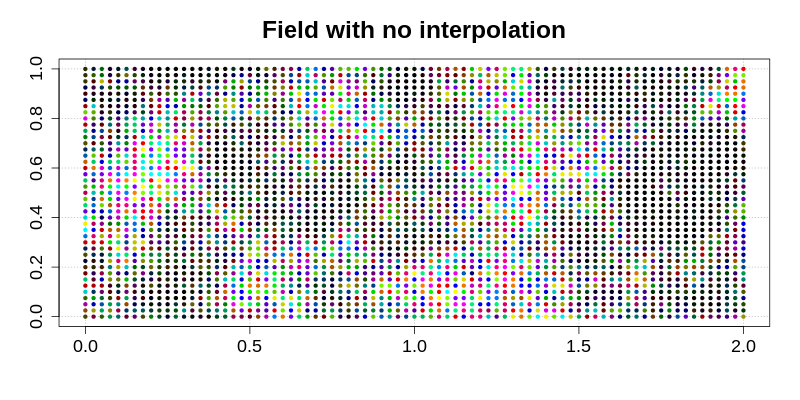
\includegraphics[width=6cm]{Figures/Field_nointerp.png}
      \caption{One field with no interpolation.}
      \label{Field1}
    \end{center}
  \end{minipage}
  \hfill
  \begin{minipage}{6cm}
    \begin{center}
      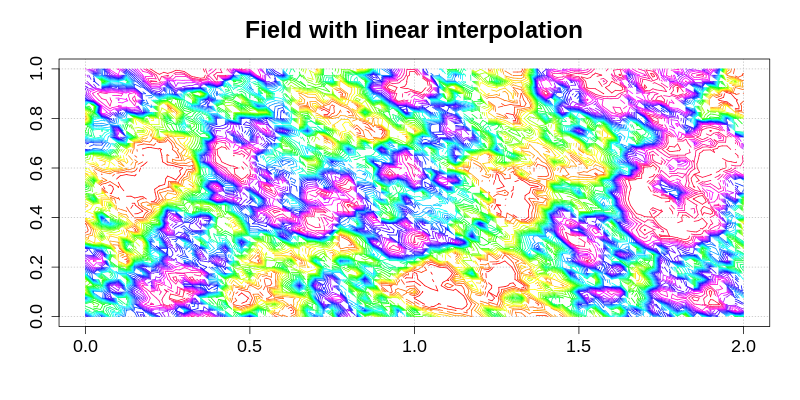
\includegraphics[width=6cm]{Figures/Field_interp.png}
      \caption{Field of Figure \ref{Field1} using linear interpolation.}
      \label{Field2}
    \end{center}
  \end{minipage}
  \hfill
  \begin{minipage}{6cm}
    \begin{center}
      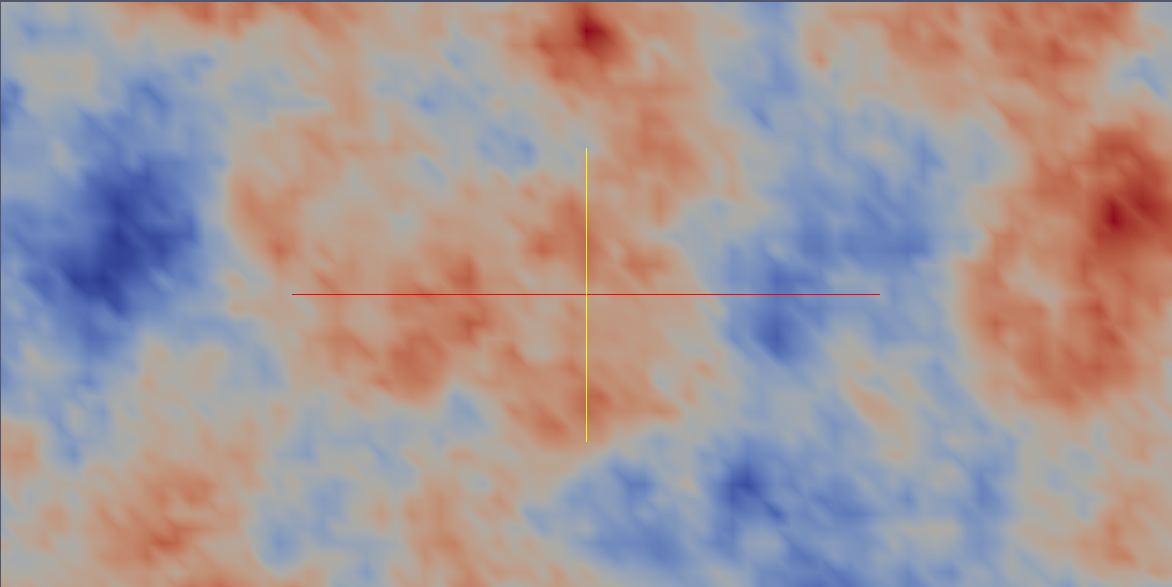
\includegraphics[width=6cm]{Figures/fieldVTK.png}
      \caption{Field of Figure \ref{Field1} visualized using ParaView.}
      \label{Field3}
    \end{center}
  \end{minipage}
\end{figure}
